\documentclass[article.tex]{subfiles}
\begin{document}

\newcommand{\Ealpha}{E_\alpha}
\newcommand{\Eedge}{E_\ell}

\section{Rationalization: Hexagon optimization}
\label{sec:regular_hexagons}

Starting from the conformal parameterization we optimize the obtained
hex-mesh to have identical regular hexagons. We use a global
optimization approach and define energies to achieve \emph{planarity},
\emph{regularity}, and \emph{equality}.

\subsubsection{Planarity.} 
The planarity function is a simple adaptation of the usual energy used
to planarize quad-meshes: A quadrilateral $\{A, B, C, D\}$ is planar
if the volume of the tetrahedron $\{A, B, C, D\}$ is zero. So if we
require the volume of all tetrahedra spanned by the vertices a polygon
to be zero we obtain a planar polygon.  The planarity energy~$\Epl$
can easily be expressed in terms of determinants.

% For a polygon~$P$ with vertices $V = \{v_1, \ldots, v_p\} \subset
% \R^3$ is given by
% \[
% \Epl(P) = \sum_{\{a,b,c,d\} \subset V} \det 
% \begin{pmatrix}
% 1 & 1 & 1 & 1 \\
% a & b & c & d
% \end{pmatrix}^2.
% \]

\subsubsection{Regularity.}
A regular planar polygon is characterized by having equal edge lengths
and equal angles at all vertices. As for planarity we define an energy
that is minimized in case of regular polygons. The interior angle at a
vertex of a regular $p$-gon is $\tfrac{p-2}{p} \pi$. So an energy $\Ereg$
that is minimized for a regular $p$-gon with vertices $\{v_1, \ldots,
v_p\}$ and corresponding angles $\{\alpha_1, \ldots, \alpha_p\}$ is
\begin{align*}
\Ereg(P) &= \lambda_P\  \Ealpha(P) + \mu_P\ \Eedge(P) &&\text{with}\\ 
\Ealpha(P) &= \sum_{i=1}^p (\alpha_i - \frac{p-2}{p} \pi)^2 
&& \Eedge(P) = \sum_{(v_i,v_{i+1})} (\|v_i - v_{i+1}\| - \ell_P)^2,
\end{align*}
where $\ell_P$ is the desired target edge length for the polygon and
$\lambda_P$ and~$\mu_P$ weights for the different energies. In a first
step, the target length can be chosen to be the average edge length of
the polygon or the shortest edge length among the edges to avoid
overlap.  Note that, the normalization of the angles already implies
planarity of the polygons.  Nevertheless, we consider the planarity
energy since it increases the rate of convergence.

Starting from a cylindrical or conical periodic conformal
parameterization we construct a hex-mesh that may or may not be
aligned with the boundary. As a consequence of the conformality of the
parameterization the angles of the hexagons are almost
$\tfrac{2\pi}{3}$. In the following we do not work with a water tight
mesh any more but split the surface into individual hexagonal
panels. We optimize the edge lengths of the hexagons to be constant
per face using~$\Eedge$. To avoid overlap we choose the length of the
shortest edge of each face as target length. We add the planarity and
angle regularity functionals~$\Epl$ and~$\Ealpha$ to the optimization
and obtain planar and regular hexagons. Each of the hexagons has its
own constant edge length. Finally, we can rationalize the panelization
further, by choosing a discrete set of edge lengths as target lengths
for the polygons in the edge length functional~$\Eedge$. Due to the
symmetry of the edge length functional for regular hexagons edge
length optimization will not destroy the planarity and regularity of
the hexagons. So it is possible to adjust the edge lengths
using~$\Eedge$ only. This quantization process is illustrated in
Figure~\ref{fig:quantization}.

\begin{figure}[tbp]
  \centering
  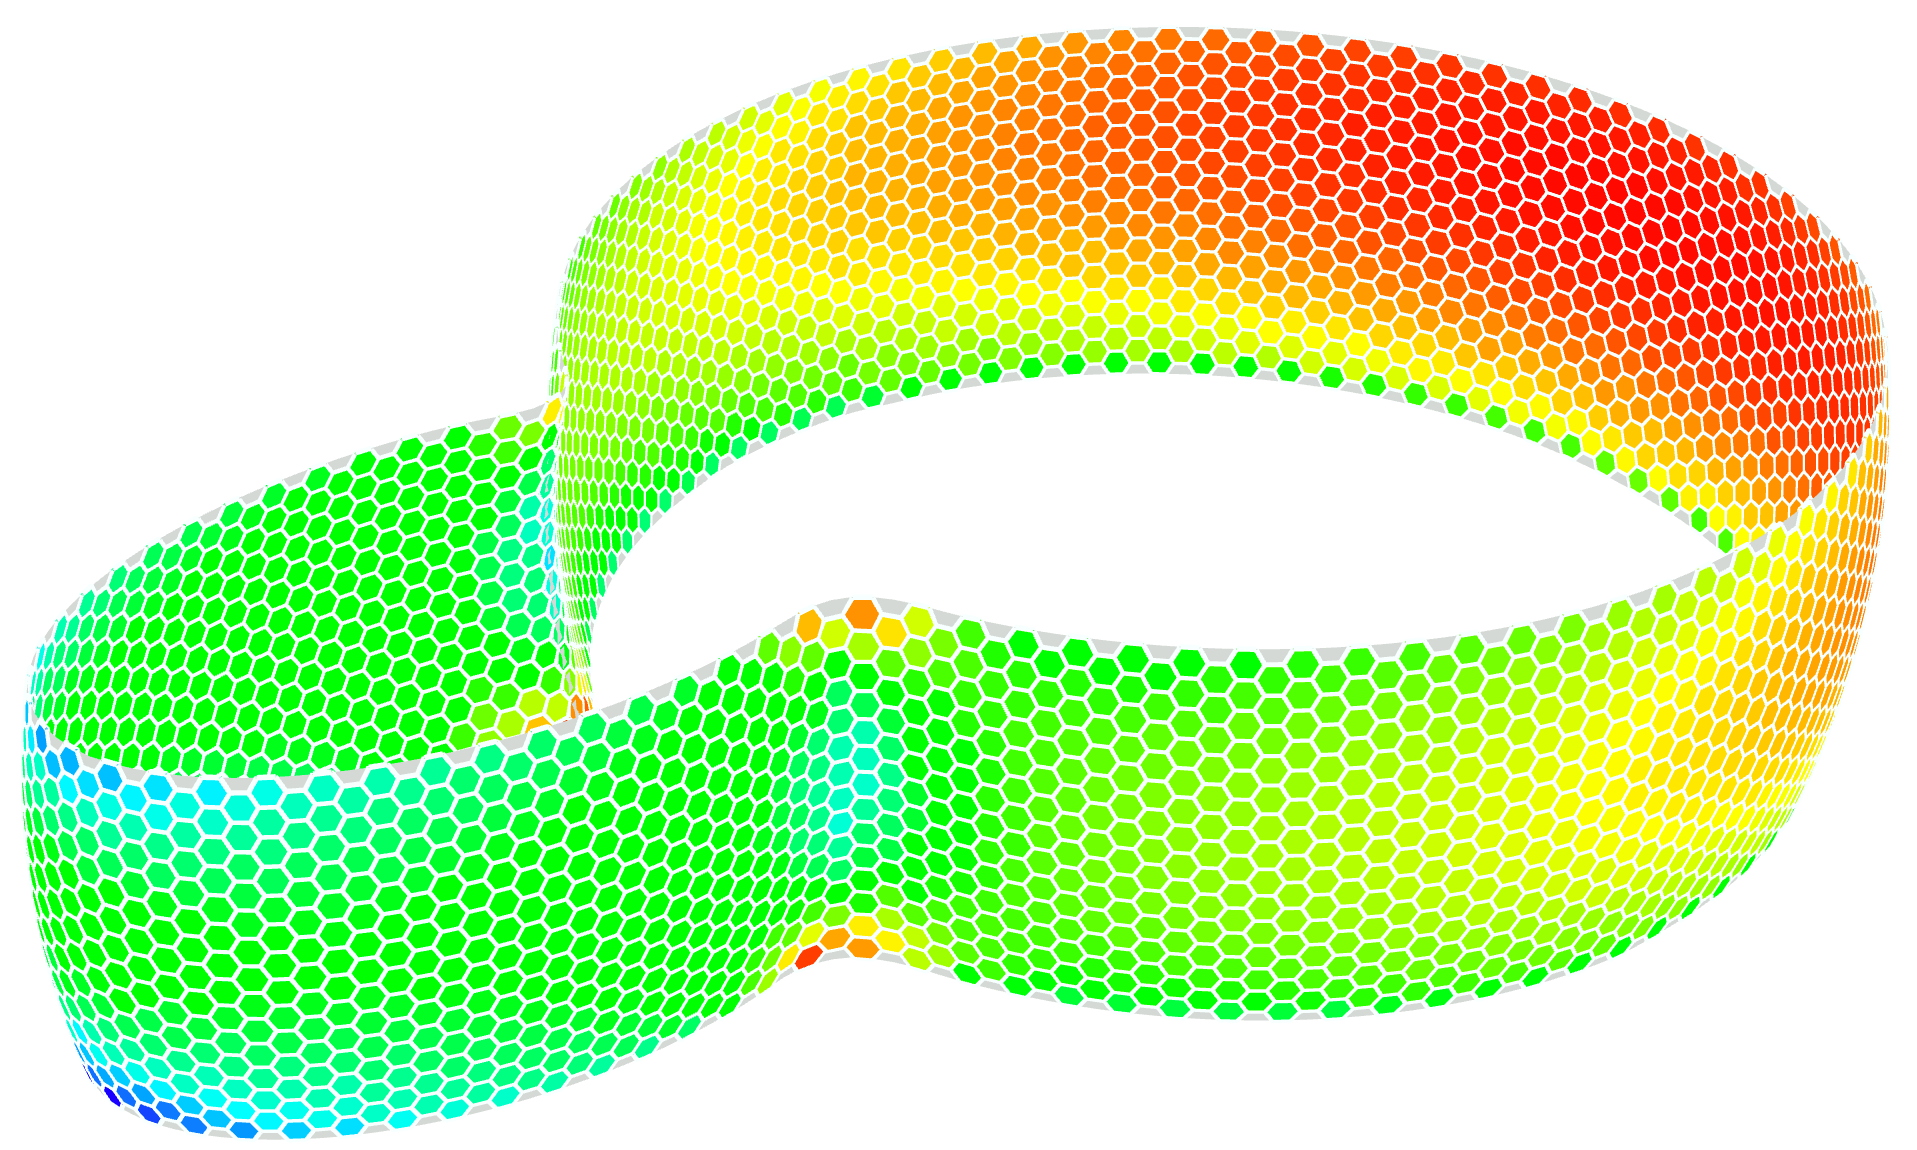
\includegraphics[width=0.48\textwidth]{images/wanda_curved_unquantized.png}
  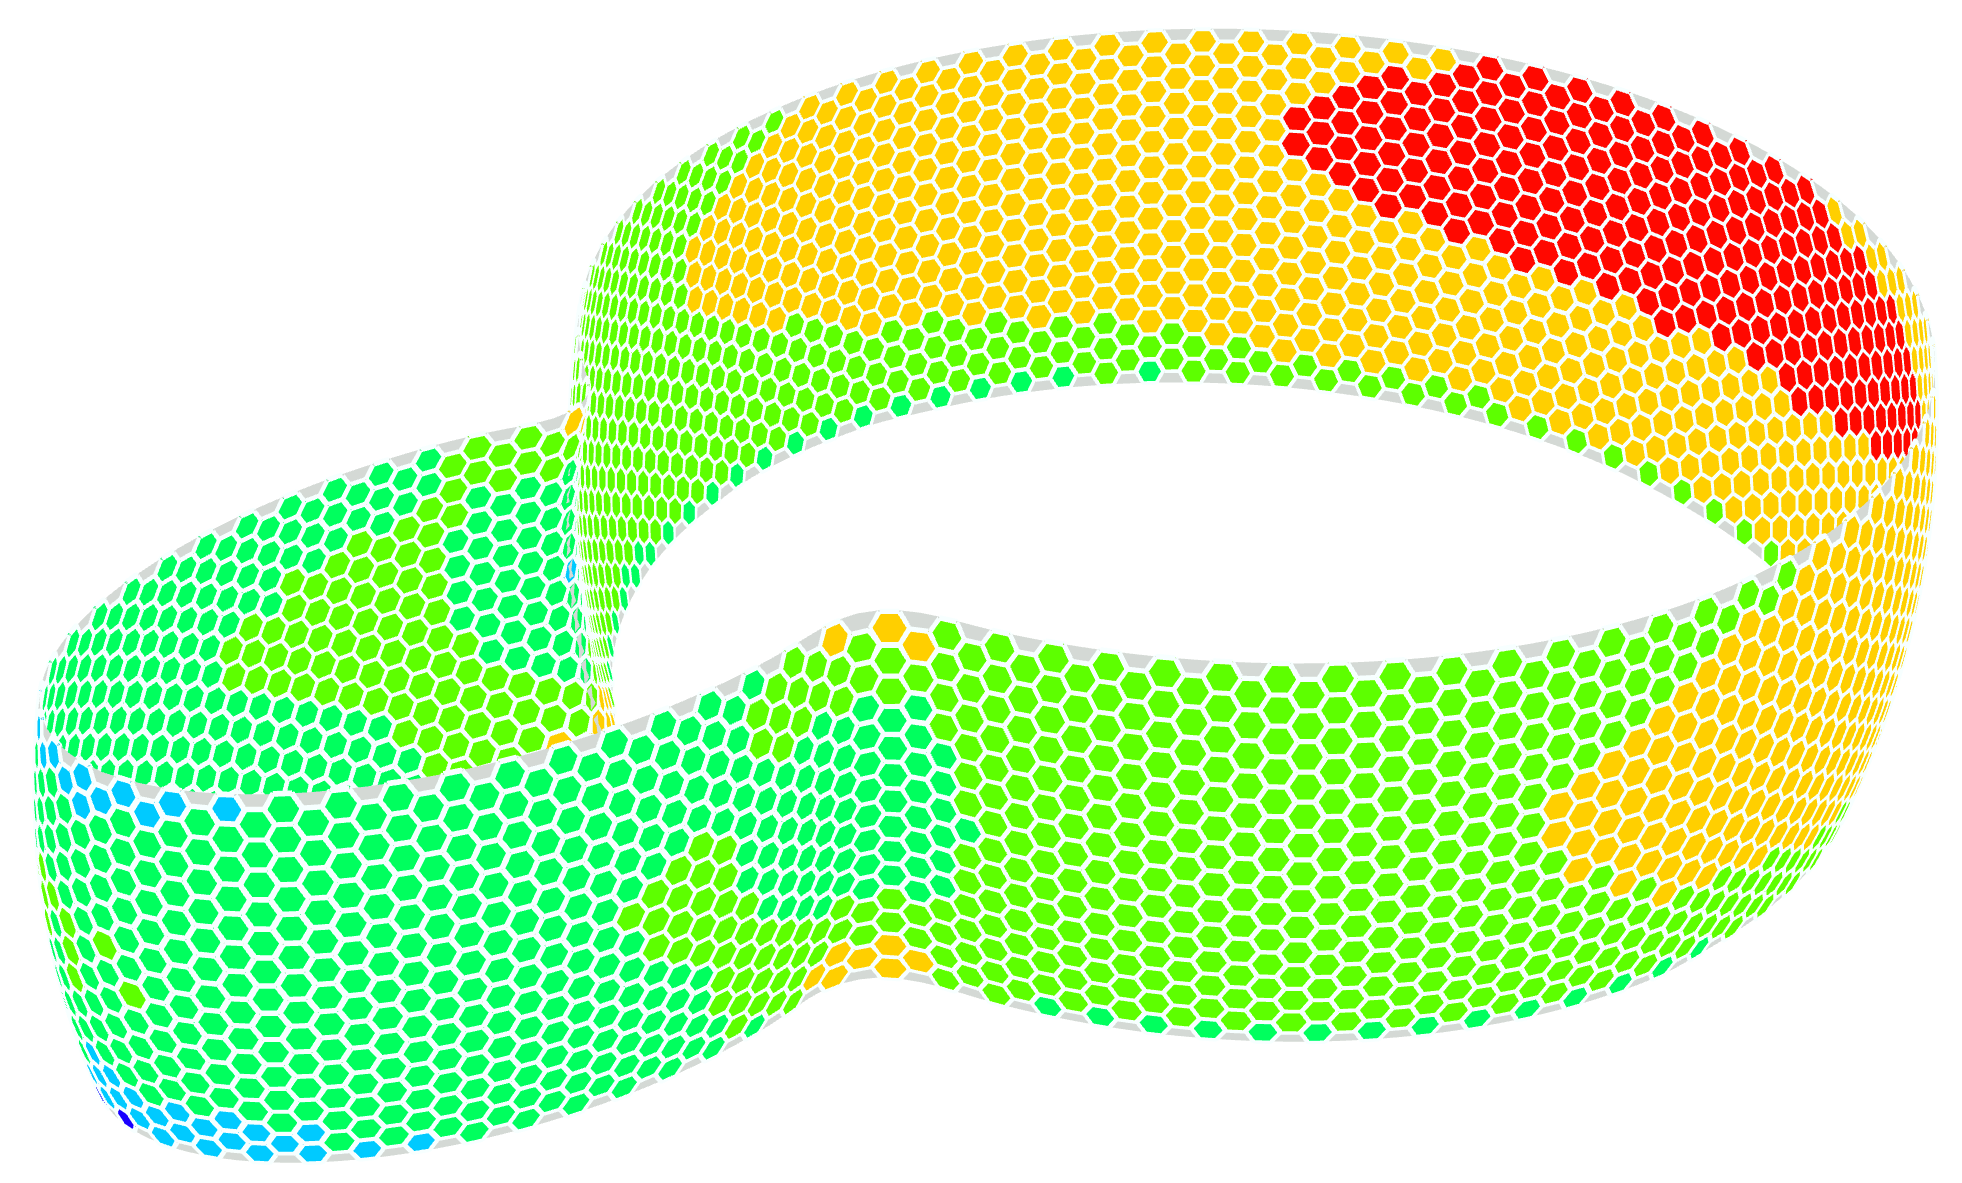
\includegraphics[width=0.48\textwidth]{images/wanda_curved_quantized.png}
  %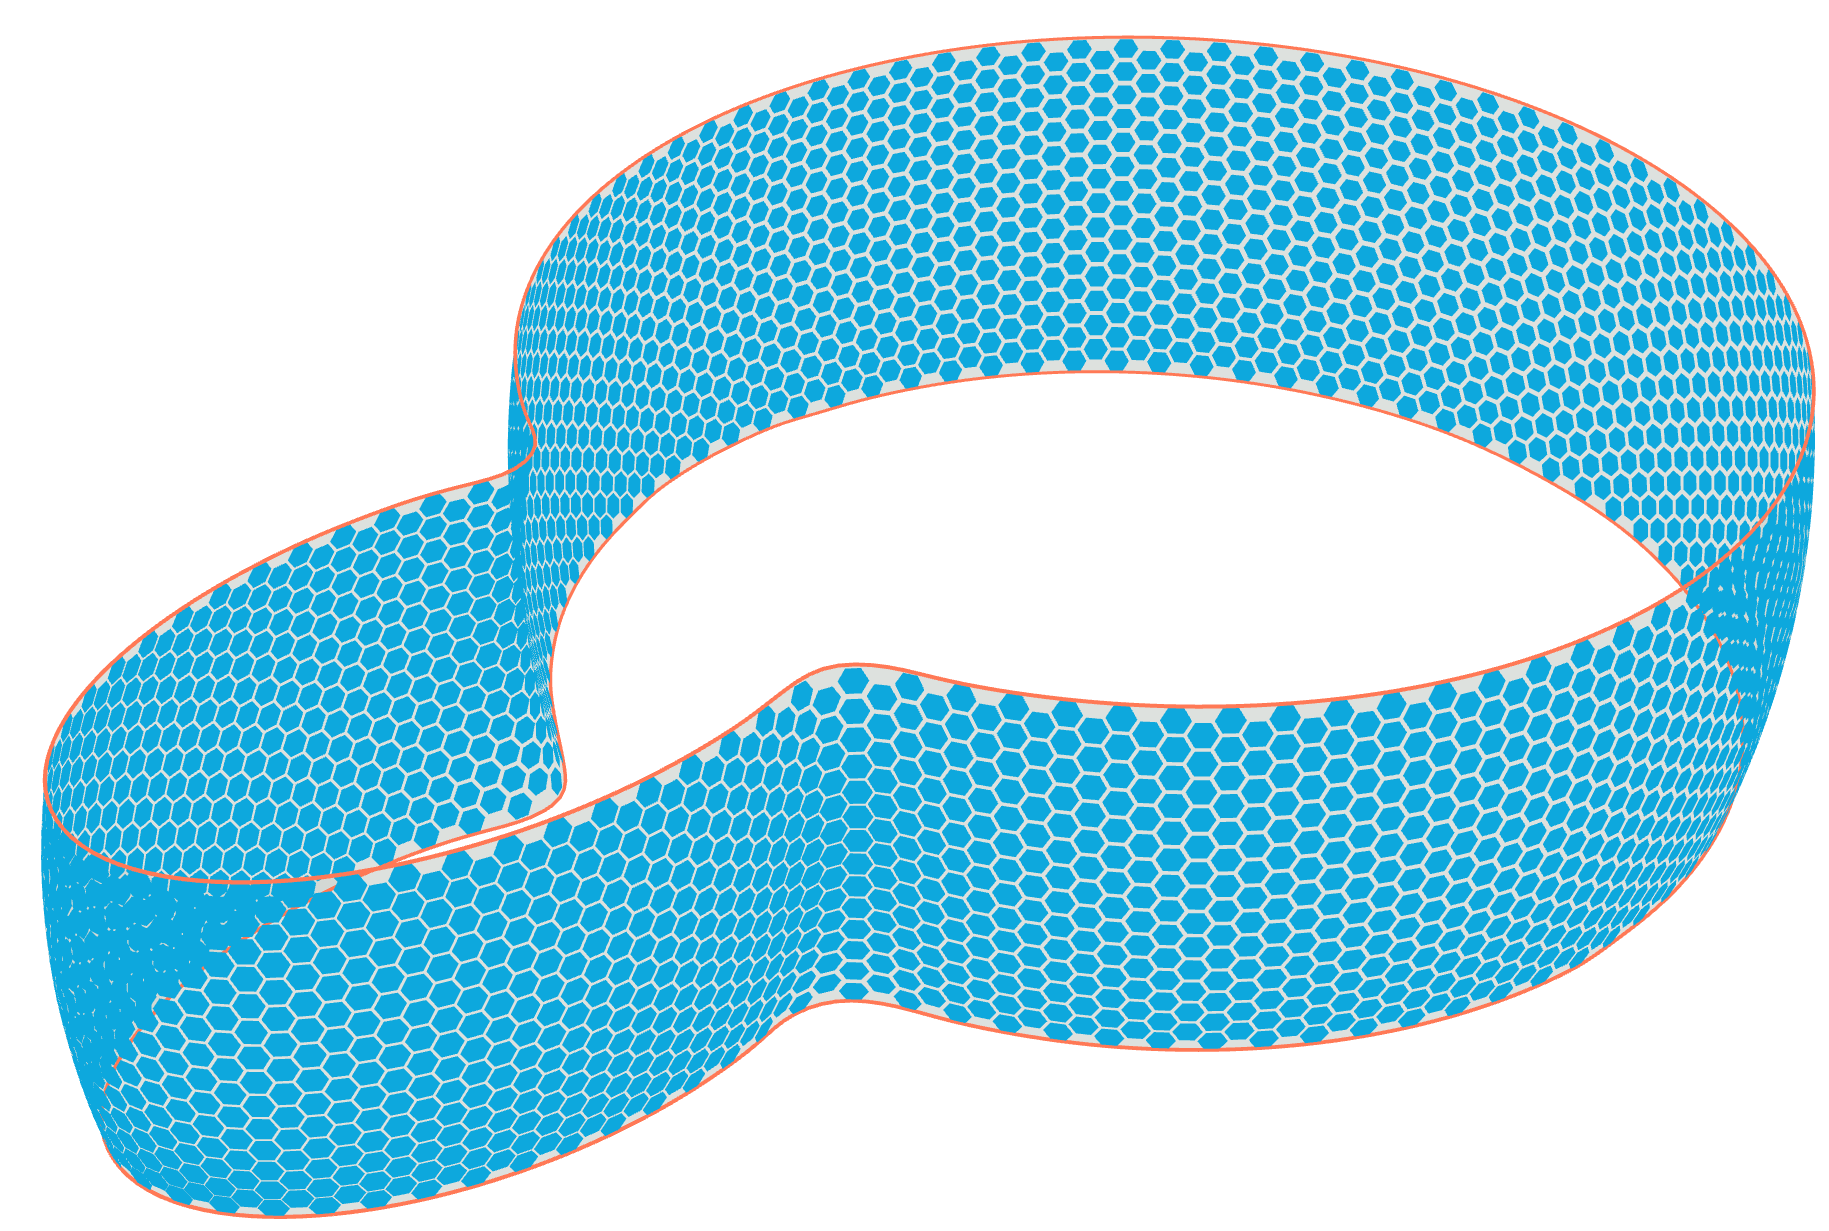
\includegraphics[width=0.3\textwidth]{images/wanda_curved_congruent.png}
  \caption{Panelization of a doubly curved design alternative of the
    case study shown in Figure~\ref{fig:overview02}. Left: Unquantized
    panelization.  Right: Quantization to $11$ panel sizes}
  \label{fig:quantization}
\end{figure}

The range of lengths obtained depends on the initial hex-mesh
constructed on the chosen target geometry. The effect of the
different periodic conformal parametrizations on the quantization is
shown in Figures~\ref{fig:cone_maps_teaser} and~\ref{fig:hex_example}.

\end{document}

%%% Local Variables: 
%%% mode: latex
%%% TeX-master: "article"
%%% End: 
